% !TEX TS–program = pdflatexmk
% !TeX program used: pdftex

\documentclass[12pt, aspectratio=169]{beamer}
% \documentclass[12pt,aspectratio=169, handout]{beamer}
\usepackage[utf8]{inputenc}
\usepackage[T1]{fontenc}
\usepackage{url}
\usepackage{graphicx}
\usepackage{subcaption}

\usepackage{amsmath, amsfonts, amssymb}
\usepackage{mathtools}

% \usetheme{Madrid}
% \usetheme{Marburg}
% \usetheme{Frankfurt}
\usetheme{Berlin}
% \useoutertheme{split}
% \setbeamertemplate{navigation symbols}{}
% \usepackage[orientation=landscape,size=custom,width=16,height=9,scale=0.5,debug]{beamerposter} 
%\usepackage{enumitem}
\usepackage{ragged2e}
\usepackage{color}
\let\olditem\item
\renewcommand\item{\olditem\justifying}
\beamertemplatenavigationsymbolsempty % Remove navigation symbols

% \usepackage[backend=biber]{biblatex}
% \usepackage[
% backend=biber,
% style=authoryear-comp,
% ]{biblatex}

\usepackage[style=authoryear,
            autocite=footnote,
            backend=biber,
           ]{biblatex}
%\bibliographystyle{ieeetr}
\addbibresource{references.bib}

\setbeamerfont{footnote}{size=\tiny} %reduce the size of the footnote citation

\setbeamertemplate{bibliography item}{\insertbiblabel}  % Add numbered list of references in the end

% \newbibmacro*{shrtcite}{%
%   \usebibmacro{cite:citepages}%
%   \iffieldundef{shorthand}
%     {\usebibmacro{cite:short}}
%     {\usebibmacro{cite:shorthand}}}

% \DeclareCiteCommand{\shrtcite}
%   {\usebibmacro{prenote}}
%   {\usebibmacro{citeindex}%
%    \usebibmacro{shrtcite}}
%   {\multicitedelim}
%   {\usebibmacro{cite:postnote}}

% \usepackage[symbol]{footmisc}
% \renewcommand{\thefootnote}{\fnsymbol{footnote}}

\AtBeginSection[]
{
    \begin{frame}
        \frametitle{Table of Contents}
        \tableofcontents[currentsection]
    \end{frame}
}

\usepackage{xcolor}

\begin{document}  
	% \author{Sam Bowyer}
	\title{Neural Simulation-Based Inference}
	%\subject{}
	%\subtitle{}
	%\logo{}
	% \institute{University of Bristol}
	\date{November 2023}
	%\setbeamercovered{transparent}
	% \setbeamertemplate{navigation symbols}{}
 
 %%%%%%%%%%%%%%%%%%%%%%%%%%%%%%%
\begin{frame}[plain]
    \vspace*{5pt}
    \vspace*{10pt}
    \maketitle
\end{frame}

 %%%%%%%%%%%%%%%%%%%%%%%%%%%%%%%

\begin{frame}{Table of Contents}
    \tableofcontents
\end{frame}

%%%%%%%%%%%%%%%%%%%%%%%%%%%%%%%
\section{Motivation}
\begin{frame}{Simulators}
    Scientists just love developing mechanistic models of phenomena:
    \begin{itemize}[<+->]
        \item Particle physics
        \item Neuroscience
        \item Population genetics
        \item Epidemiology
        \item Climate/Earth sciences
        \item Astrophysics
    \end{itemize}

    \pause 
    Thanks to modern computing, they can turn these into high-precision simulators.
\end{frame}

%%%%%%%%%%%%%%%%%%%%%%%%%%%%%%%
\begin{frame}{Simulators: An Example}
    Geant4 - particle simulator \parencite{cern_geant4_nodate}.
    
    % Too complicated to get tractable likelihood (latent space $\mathcal{Z}$ is massive).

    \begin{columns}
		\begin{column}{0.5\textwidth}
		\begin{figure}
			\centering
			
\includegraphics[width=0.8\linewidth]{"images/geant4_logo.png"}\label{fig:g4_logo}
		\end{figure}
		\end{column}
			
		\begin{column}{0.5\textwidth}
		\begin{figure}
			\centering
			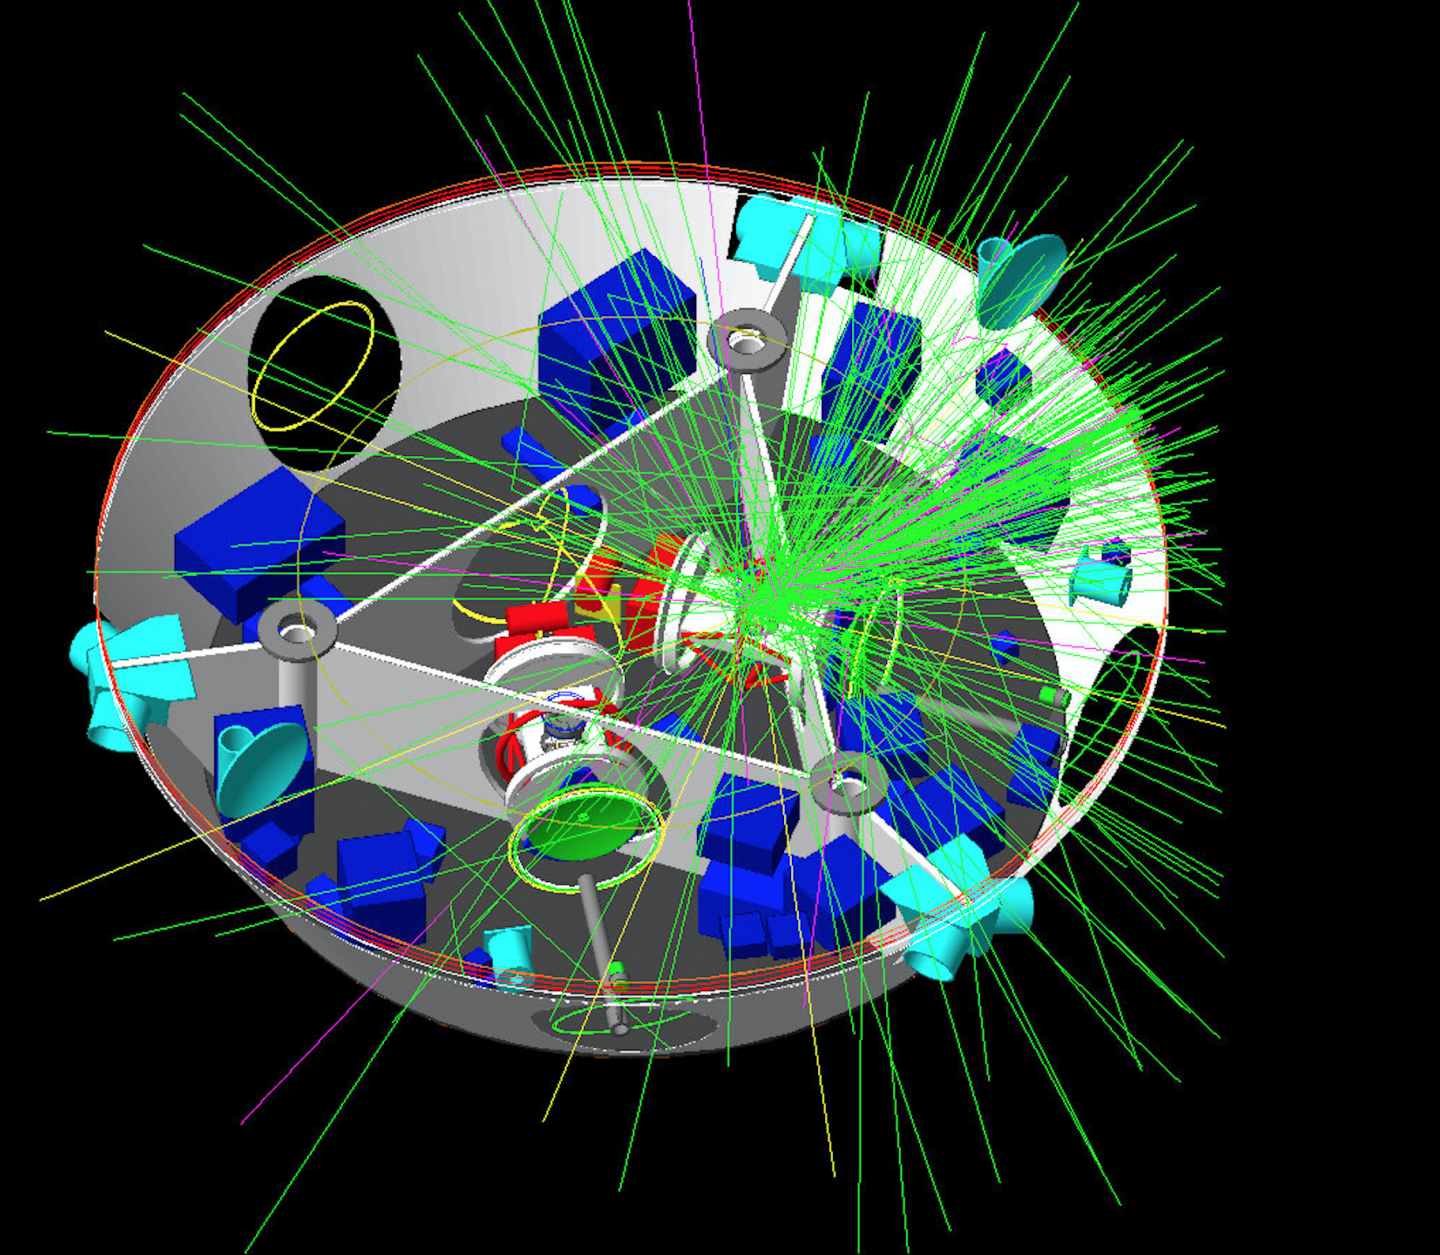
\includegraphics[width=0.75\linewidth]{"images/geant4.png"}\label{fig:g4}
		\end{figure}
		\end{column}
	\end{columns}
\end{frame}

%%%%%%%%%%%%%%%%%%%%%%%%%%%%%%%
\begin{frame}{Science (like, most of it)}   
    \begin{figure}
		\centering
		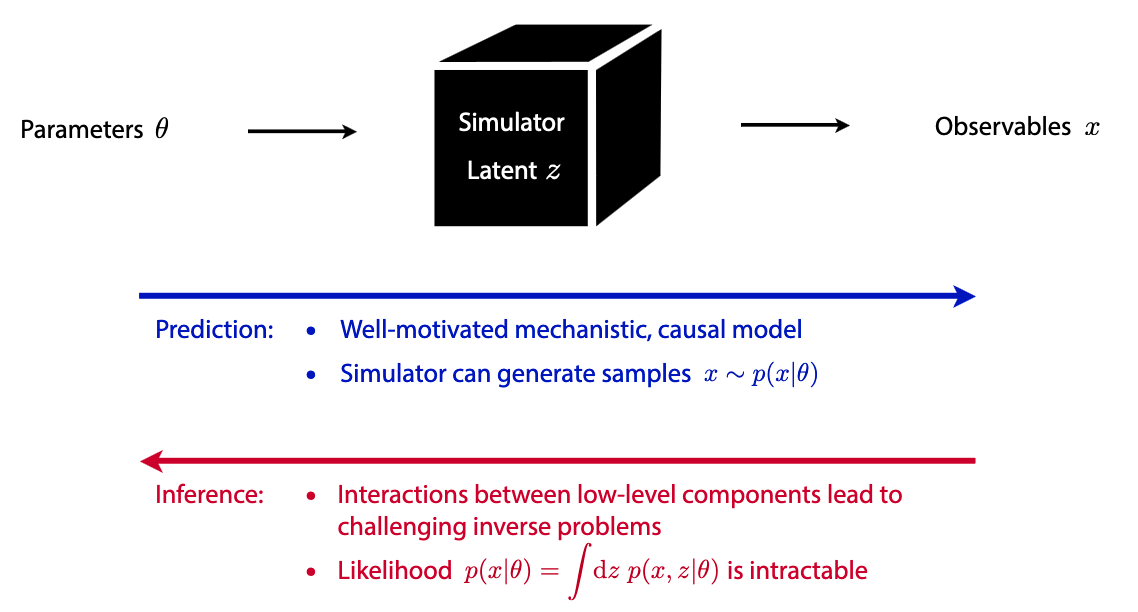
\includegraphics[width=0.7\textwidth]{"images/science.png"}
        \caption{Credit: Johann Brehmer \parencite{brehmer_slides2022simulation_based_inference_rodem_sinergia_2022pdf_2022}.}
	\end{figure}
\end{frame}

% %%%%%%%%%%%%%%%%%%%%%%%%%%%%%%%
% \begin{frame}{Simulators: An Example}
%     Geant4 - particle simulator \parencite{cern_geant4_nodate}.
    
%     Too complicated to get tractable likelihood (latent space $\mathcal{Z}$ is massive).

%     \begin{columns}
% 		\begin{column}{0.5\textwidth}
% 		\begin{figure}
% 			\centering
% 			
\includegraphics[width=0.8\linewidth]{"images/geant4_logo.png"}\label{fig:g4_logo}
% 		\end{figure}
% 		\end{column}
			
% 		\begin{column}{0.5\textwidth}
% 		\begin{figure}
% 			\centering
% 			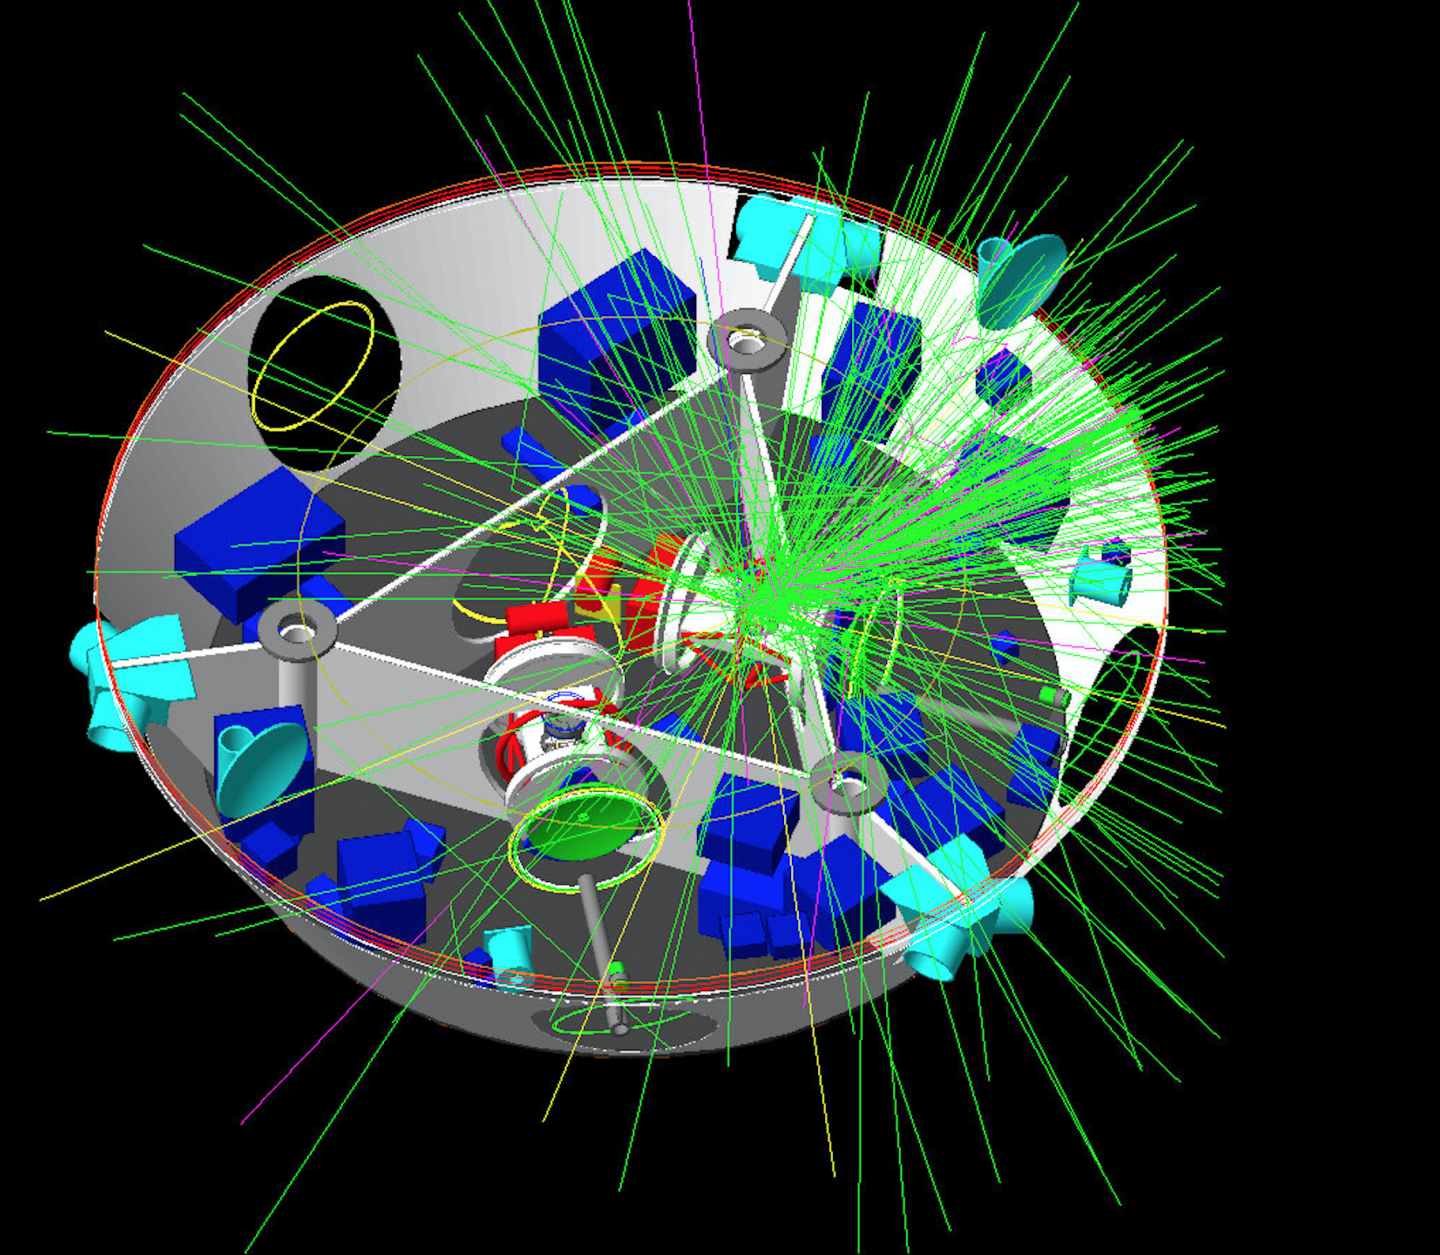
\includegraphics[width=0.75\linewidth]{"images/geant4.png"}\label{fig:g4}
% 		\end{figure}
% 		\end{column}
% 	\end{columns}
% \end{frame}

%%%%%%%%%%%%%%%%%%%%%%%%%%%%%%%
\begin{frame}{Likelihood-Free Inference}
\alert{The Problem: } Performing inference over parameters $\theta$ with data $x$

$$p(\theta | x) = \frac{p(x | \theta) p(\theta)}{p(x)}$$

when we don't have access to the likelihood $p(x|\theta)$, but we can sample $x \sim p(x|\theta)$.


\end{frame}


%%%%%%%%%%%%%%%%%%%%%%%%%%%%%%%
\section{Traditional Methods}
\begin{frame}{Traditional Methods: Summary Statistics}

    \begin{columns}
		\begin{column}{0.45\textwidth}
        \begin{itemize}
            \item Choose a good summary statistic $s(x)$ based on domain knowledge (feature engineering)---this is \textit{hard}.
            
            \pause
            
            \item Approximate the likelihood $p(s|\theta)$ using histograms or kernel density estimation (e.g. \cite{diggle_monte_1984}).

            \pause 
            
            \item Does not scale well with the dimension of $s(x)$.
        \end{itemize}
        
        \end{column}

        \pause

        \begin{column}{0.55\textwidth}
            \begin{figure}
    			\centering
    			\includegraphics[width=0.75\linewidth]{"images/atlas_histogram.png"}\label{fig:g4}
            \end{figure}
            \vspace{-0.98em}
            Essentially what was used for the Higgs boson discovery \parencite{atlas_collaboration_observation_2012}.
        \end{column}
    \end{columns}

\end{frame}

%%%%%%%%%%%%%%%%%%%%%%%%%%%%%%%
\begin{frame}{Traditional Methods: Approximate Bayesian Computation}

\begin{columns}
    \begin{column}{0.6\textwidth}
        Given true observed data $x_o$, want to find a set of suitable parameters $\theta \sim p(\theta | x_o)$.
        \begin{enumerate}[<+->]
            \item Sample $\theta \sim p(\theta)$.
            \item Simulate $x \sim p(x | \theta)$.
            \item Calculate summary statistics $s(x_o)$ and $s(x)$.
            \item Accept $\theta$ if the distance $\rho(s(x_o), s(x)) \leq \epsilon$, reject otherwise.
            \item Repeat.
        \end{enumerate}
         \parencite{rubin_bayesianly_1984}
    \end{column}
    
    \begin{column}{0.4\textwidth}
        \begin{figure}
            \centering
            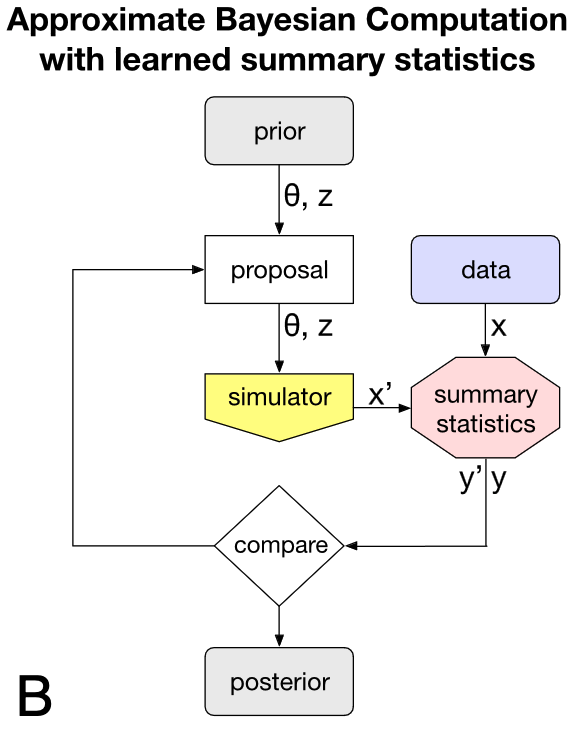
\includegraphics[height=0.62\textheight]{"images/ABC_s2.png"}
            \caption{\cite{cranmer_frontier_2020}}
        \end{figure}
    \end{column}
\end{columns}

\pause

Two obvious problems: (1) How to choose $\rho, \epsilon$? (2) This is very slow for small $\epsilon$.

\end{frame}

%%%%%%%%%%%%%%%%%%%%%%%%%%%%%%%
\begin{frame}{Problems with ABC}

Three main problems:
\begin{enumerate}[<+->]
    \item Choosing $s(x)$ to be informative and low-dimensional.
    \item Choosing $\rho$ and $\epsilon$.
    \item Tends to be very slow for small $\epsilon$. 
    \begin{itemize}
        \item (Simulation is typically the bottleneck in SBI.)
    \end{itemize}
\end{enumerate}
\end{frame}

% %%%%%%%%%%%%%%%%%%%%%%%%%%%%%%%
% \begin{frame}{Problems with ABC \& Summary Statistics}
%     \begin{enumerate}
%         \item Require lots of domain knowledge and choice of $s, \rho, \epsilon$.
%         \item Slow (in terms of # simulations).
%     \end{enumerate}

%     \pause 
%     Late 2010s: people start applying methods from deep learning to SBI.

% \end{frame}


%%%%%%%%%%%%%%%%%%%%%%%%%%%%%%%
\begin{frame}{Modern Simulation-Based Inference}
	\begin{figure}
		\centering
		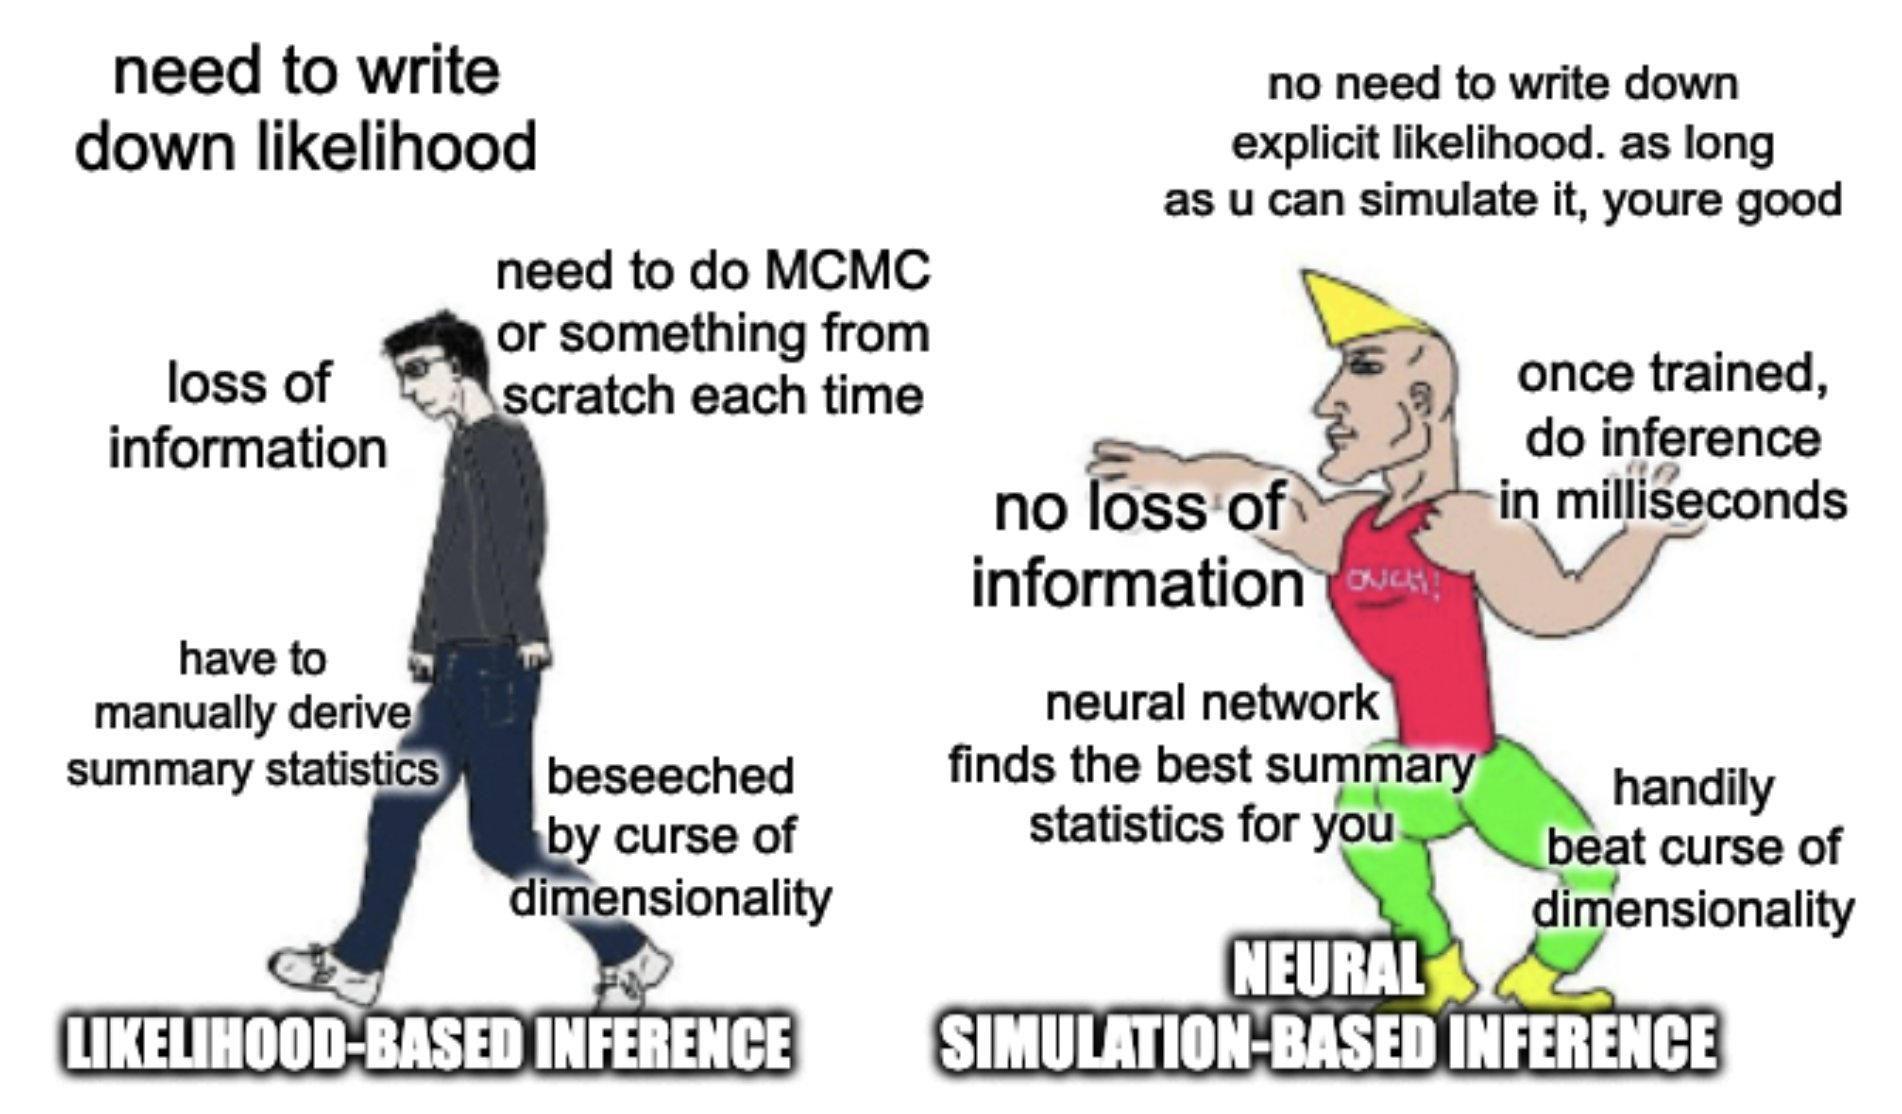
\includegraphics[width=0.75\textwidth]{"images/sbi.jpeg"}
	\end{figure}
	% \footfullcite{ray2018survey}	
\end{frame}

%%%%%%%%%%%%%%%%%%%%%%%%%%%%%%%
\begin{frame}{Using Neural Networks}
    Two main approaches to Neural SBI:
    \begin{enumerate}
        \item Supervised Learning: Use NN to model a likelihood ratio (NRE)
        $$r(x | \theta) \vcentcolon= \frac{p(x|\theta)}{p_{\text{ref}}(x)} \text{ or } r(x | \theta_0, \theta_1) \vcentcolon = \frac{p(x|\theta_0)}{p(x|\theta_1)}$$
        
        \pause
        \item Unsupervised Learning: Use conditional neural density estimates (e.g. normalizing flows)
        \begin{itemize}
            \item Neural Posterior Estimation (NPE): Model $p(\theta | x)$
            \item Neural Likelihood Estimation (NLE): Model $p(x|\theta)$
        \end{itemize}
    \end{enumerate}
\end{frame}

%%%%%%%%%%%%%%%%%%%%%%%%%%%%%%%
\section{Using Classifiers (NRE)}
\begin{frame}{Neural Likelihood Ratio Estimation (NRE)}
    \alert{Neyman-Pearson lemma} \parencite{neyman_ix_1933}: The most powerful test statistic to compare two hypotheses $\theta_0$ and $\theta_1$ for an observation $x$ is the likelihood ratio:

    $$r(x | \theta_0, \theta_1) \vcentcolon=\frac{p(x|\theta_0)}{p(x|\theta_1)}$$
    
\end{frame}

%%%%%%%%%%%%%%%%%%%%%%%%%%%%%%%
\begin{frame}{NRE: Likelihood Ratio Trick}
    Use supervised learning to obtain a classifier $\mathbf{d}(x)$ to distinguish between
    \begin{itemize}
        \item $x \sim p (x | \theta_0)$ with class label $y=1$, and
        \item $x \sim p (x | \theta_1)$ with class label $y=0$.
    \end{itemize}

    \pause 
    This has optimal classifier
    $$\mathbf{d}^*(x) = p(y=1 | x) = \frac{p(x|\theta_0)}{p(x|\theta_0) + p(x|\theta_1)}$$
    \pause 
    Which can be used to obtain the likelihood ratio
    $$r(x|\theta_0, \theta_1) = \frac{p(x|\theta_0)}{p(x|\theta_1)} = \frac{\mathbf{d}^* (x)}{1-\mathbf{d}^*(x)}$$.
\end{frame}

%%%%%%%%%%%%%%%%%%%%%%%%%%%%%%%
\begin{frame}{NRE: Parameterized Classifier}
    Clearly we can't train a new classifier $\mathbf{d}$ for every possible pair of $\theta_0, \theta_1 \in \Theta$.

    \pause 

    \begin{columns}

        \begin{column}{0.5\textwidth}
            \begin{itemize}[<+->]
                \item So train a `parameterised classifier'\footnote[*]{\textsuperscript{*}\parencite{cranmer_approximating_2016, hermans_likelihood-free_2020}} $\mathbf{d}(x, \theta)$ that takes in a proposed $\theta$ as input.
                % \pause
                \item Try to target the likelihood ratio against some reference $p_\text{ref}(x)$
                $$r(x | \theta) = \frac{p(x|\theta)}{p_{\text{ref}}(x)}$$

            \end{itemize}
        
        \end{column}

        % \pause 
        
		\begin{column}{0.5\textwidth}
            \begin{figure}
        		\centering
        		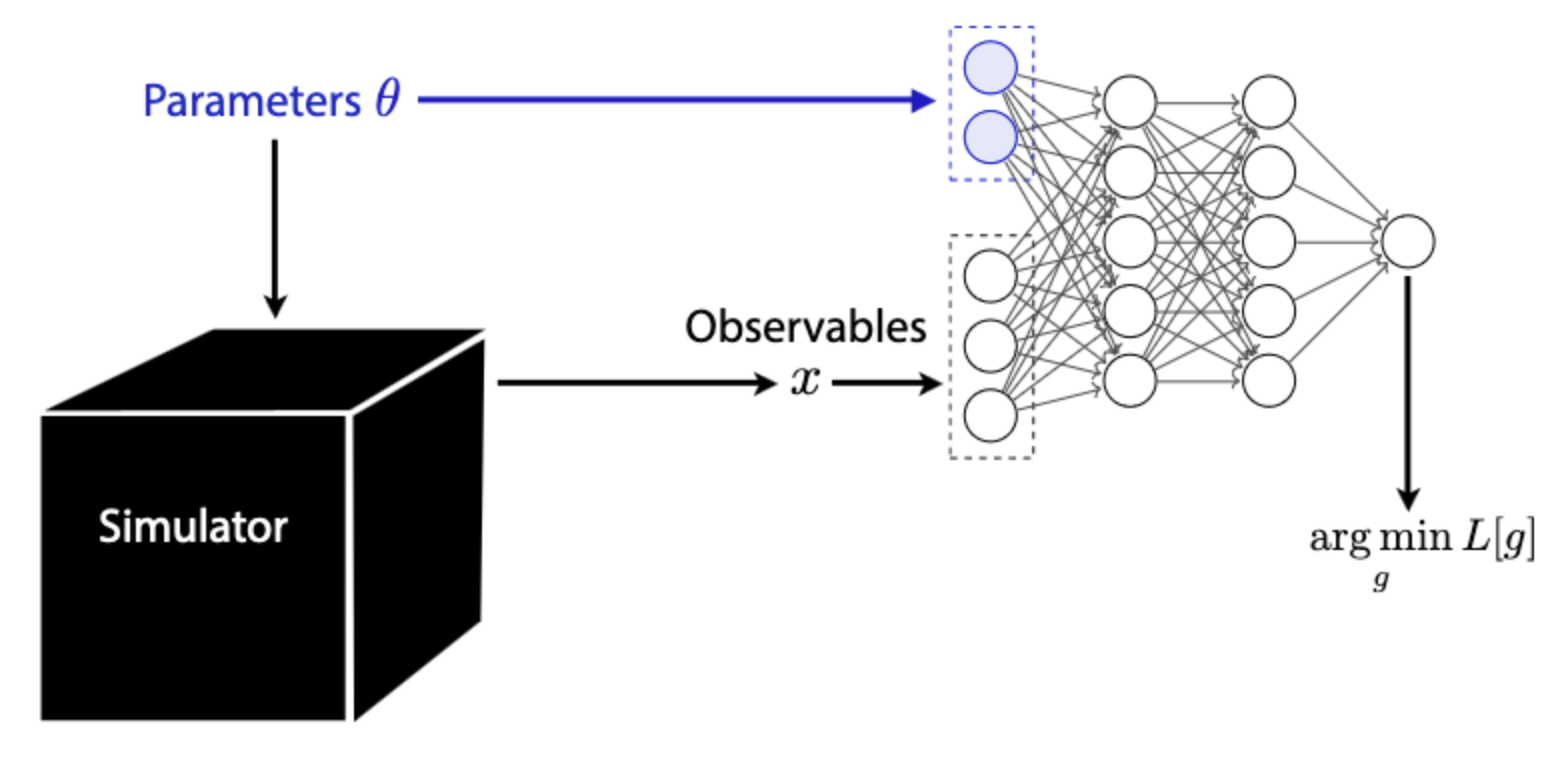
\includegraphics[width=0.8\textwidth]{"images/parameterised_classifier.png"}
                \caption{Credit: Johann Brehmer \parencite{brehmer_slides2022simulation_based_inference_rodem_sinergia_2022pdf_2022}.}
    	    \end{figure}
        \end{column}
    \end{columns}
    
\end{frame}

%%%%%%%%%%%%%%%%%%%%%%%%%%%%%%%
\begin{frame}{NRE: Parameterized Classifier}

    \begin{itemize}
        \item In particular, train parameterised classifier $\mathbf{d}(x, \theta)$ to distinguish between 
        \begin{enumerate}
            \item dependent $(x,\theta) \sim p(x, \theta)$ pairs with class label $y=1$, 
                $$\theta \sim p(\theta), \;\;\; x \sim p(x|\theta)$$
            \item independent $(x, \theta')$ pairs with class label $y=0$
                $$\theta' \sim p(\theta)$$
        \end{enumerate}
    
        \pause 
        
        \item This gives us the optimal classifier 
        $$\mathbf{d}^*(x, \theta) = p(y=1 | x, \theta) = \frac{p(x,\theta)}{p(x,\theta) + p(x)p(\theta)}$$

    \end{itemize}
\end{frame}

%%%%%%%%%%%%%%%%%%%%%%%%%%%%%%%
\begin{frame}{NRE: Parameterized Classifier} 
    With this optimal classifier
    $$\mathbf{d}^*(x, \theta) = p(y=1 | x, \theta) = \frac{p(x,\theta)}{p(x,\theta) + p(x)p(\theta)}$$

    \pause 
    
    the likelihood trick gives us:

    $$\frac{\mathbf{d}^*(x, \theta)}{1-\mathbf{d}^*(x, \theta)} = \frac{p(x,\theta)}{p(x)p(\theta)} = \frac{p(x|\theta)}{p(x)} = r(x|\theta)$$

    i.e. we're implicitly using $p_\text{ref}(x) = p(x)$.
\end{frame}

%%%%%%%%%%%%%%%%%%%%%%%%%%%%%%%
\begin{frame}{NRE: Algorithm Psuedocode}
    \begin{columns}
        \begin{column}{0.5\textwidth}
            \begin{figure}
                \centering
                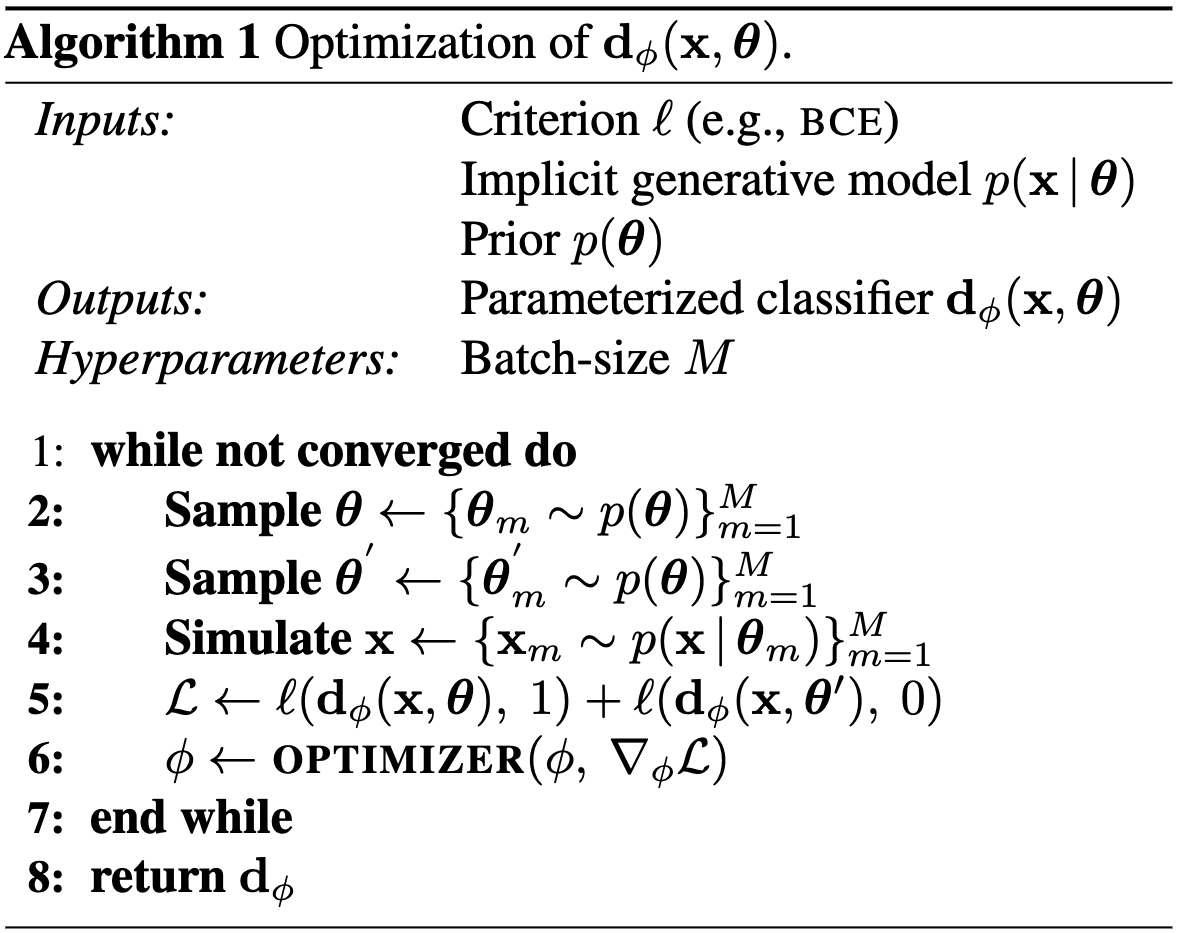
\includegraphics[height=0.6\textheight]{"images/NRE_algo2.png"}
                \caption{\cite{hermans_likelihood-free_2020}}
            \end{figure}
        \end{column}

        \begin{column}{0.5\textwidth}
            \begin{figure}
                \centering
                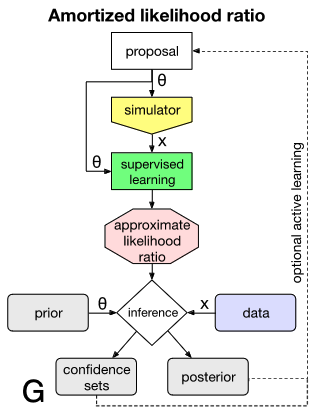
\includegraphics[height=0.6\textheight]{"images/SNRE.png"}
                \caption{\cite{cranmer_frontier_2020}}
            \end{figure}
        \end{column}
    \end{columns}
\end{frame}

%%%%%%%%%%%%%%%%%%%%%%%%%%%%%%%
\begin{frame}{NRE: Algorithm Diagram}
    \begin{figure}
		\centering
		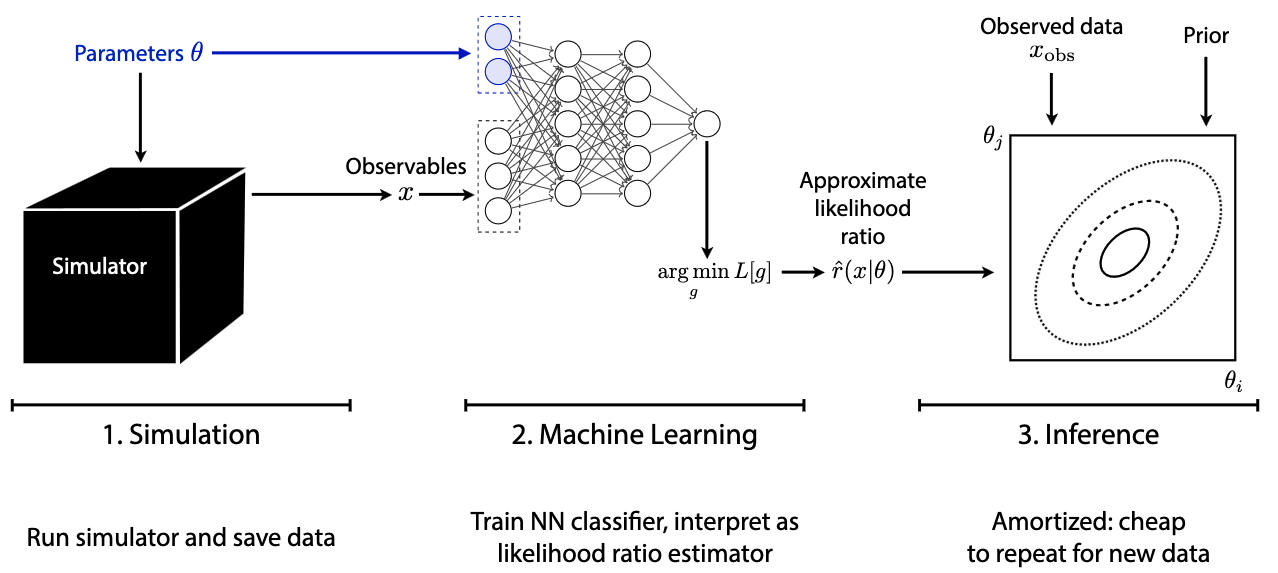
\includegraphics[width=0.83\textwidth]{"images/NRE_diagram.png"}
        \caption{\cite{hermans_likelihood-free_2020}}
	\end{figure}
\end{frame}

%%%%%%%%%%%%%%%%%%%%%%%%%%%%%%%
\begin{frame}{NRE: Inference}
    \begin{itemize}
        \item Frequentist: Run for a whole lot of values of $\theta$ and get some confidence intervals.
        
        \pause 
        
        \item Bayesian:
        \begin{itemize}
            \item Metropolis-Hastings MCMC
            $$\alpha = \min \left(1, \frac{p(\theta') \textcolor{red}{p(x|\theta')}q(\theta'|\theta_t)}{p(\theta_t)\textcolor{red}{p(x|\theta_t)}q(\theta_t|\theta')}\right)$$
            \item Hamiltonian Monte Carlo
            $$\nabla_\theta U(\theta) = - \frac{\nabla_\theta p(x|\theta)}{p(x|\theta)}$$.
        \end{itemize}
    \end{itemize}
\end{frame}

% %%%%%%%%%%%%%%%%%%%%%%%%%%%%%%%
% \begin{frame}{NRE: Sampling from the Posterior}
%     % [GET SCREENSHOT] of Fig 7 in hermans 2020 of Einstein radius $\theta \in \mathbb{R}$ gravitational lensing (nice cool example)
%     \begin{figure}
% 		\centering
% 		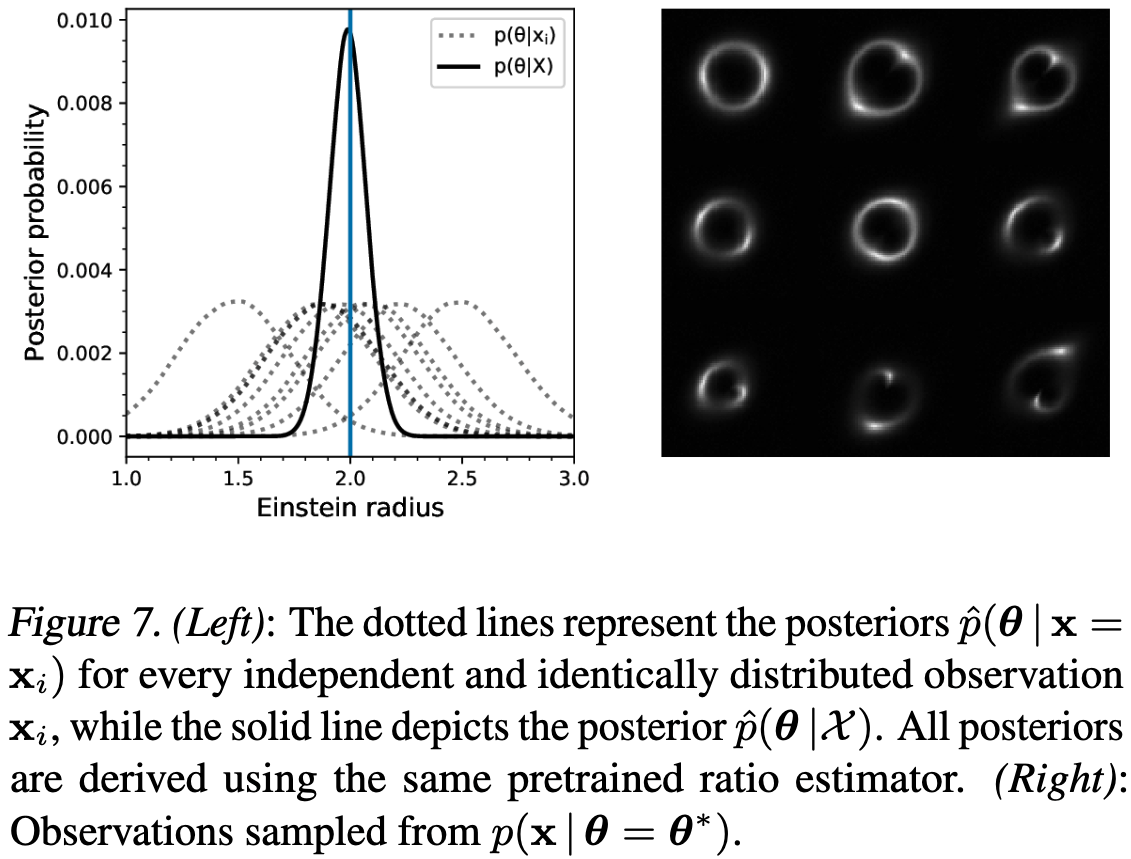
\includegraphics[width=0.45\textwidth]{"images/SNRE_results2.png"}
%         \caption{\cite{hermans_likelihood-free_2020}}
% 	\end{figure}
% \end{frame}

%%%%%%%%%%%%%%%%%%%%%%%%%%%%%%%
\section{Neural Density Estimation (NPE \& NLE)}
\begin{frame}{Conditional Neural Density Estimation}
    \begin{itemize}[<+->]

        \item Train a NN $q_\phi$ to learn a density $p(u|v)$, given iid pairs $\{(u_i,v_i)\}_{i=1}^n$ from the joint distribution $p(u,v)$ by maximising the total log probability w.r.t. $\phi$
        $$\sum_{i=1}^n \log q_\phi(u_i|v_i)$$

    \end{itemize}
\end{frame}

%%%%%%%%%%%%%%%%%%%%%%%%%%%%%%%
\begin{frame}{Conditional Neural Density Estimation: Mixture Density Networks}
    \begin{itemize}[<+->]

        \item Mixure Density Network (MDN): $q_\phi(u|v)$ is a mixture of $K$ Gaussians:
        $$q_\phi(u|v) = \sum_{k=1}^K \alpha_k \mathcal{N}(u | \mu_k, \Sigma_k)$$
        where $\{\alpha_k\}, \{\mu_k\}, \{\Sigma_k\}$ are computed by a feed-forward NN.
        \begin{itemize}
            \item Not very popular anymore (used in \cite{papamakarios_fast_2018}), but nice and simple (and easily normalised).
        \end{itemize}
        
    \end{itemize}
\end{frame}

%%%%%%%%%%%%%%%%%%%%%%%%%%%%%%%
\begin{frame}{Conditional Neural Density Estimation: Normalising Flows}
    \begin{itemize}[<+->]
        \item Normalising Flow: $q_\phi(u|v)$ is a transformation of a standard Gaussian density $\mathcal{N}(0,\mathbf{I})$ through a series of $K$ invertible, differentiable functions $f_1, \ldots, f_K$ which each depend on $v$, i.e.:
        % \begin{align}
        % z_0 &\sim \mathcal{N}(0, \mathbf{I}) \\
        % z_k &= f_k(z_{k-1}, \theta) \\
        % x &= z_K
        % \end{align}
        $$ z_0 \sim \mathcal{N}(0, \mathbf{I}), \;\;\; z_k = f_k(z_{k-1}, v) \in \mathbb{R}^M, \;\;\; u = z_K$$

        \item By a change of variables we get that
        $$q_\phi(u|v) = \mathcal{N}(z_0|0, \mathbf{I}) \prod_{k=1}^K \left|\det \left(\frac{\partial f_k}{\partial z_{k-1}}\right) \right|^{-1}.$$

        % \begin{itemize}
            \item One choice is a Masked Autoregressive Flow (MAF) \parencite{papamakarios_masked_2018}.
            % where each $f_k$ is a Masked Autoencoder for Distribution Estimation (MADE) \parencite{germain_made_2015}.
            % \item One choice is for a Masked Autoregressive Flow (MAF) \parencite{papamakarios_masked_2018} where each $f_k$ 
            
            % (using a Masked Autoencoder for Distribution Estimation (MADE) \parencite{germain_made_2015}).
        % \end{itemize}
        
    \end{itemize}
\end{frame}

%%%%%%%%%%%%%%%%%%%%%%%%%%%%%%%
\begin{frame}{Normalising Flows: MAF}
    % $$ z_0 \sim \mathcal{N}(0, \mathbf{I}), \;\;\; z_k = f_k(z_{k-1}, \theta), \;\;\; x = z_K$$
    % $$q_\phi(u|v) = \mathcal{N}(z_0|0, \mathbf{I}) \prod_{k=1}^K \left|\det \left(\frac{\partial f_k}{\partial z_{k-1}}\right) \right|^{-1}.$$
    
    % \pause
    
    \begin{itemize}[<+->]
        \item Each component $z_k^{(j)}$ is computed depending on the previous components $z_k^{(1)}, \ldots, z_k^{(j-1)}$:

        $$p(z_k^{(j)} | z_k^{(1:j)}) = \mathcal{N}(z_k^{(j)} | \mu_k^{(j)}, (\exp\alpha_k^{(j)})^2)$$
        where
        % $$\mu_k^{(j)} = f_k^{\mu_k^{(j)}}(z_k^{(1:j-1)}) \text{ and } \alpha_k^{(j)} = f_k^{\alpha_k^{(j)}}(z_k^{(1:j-1)}).$$
        $\mu_k^{(j)}$ and $\alpha_k^{(j)}$ come from the NN receiving $z_k^{(1:j-1)}$ and $v$ as input.

        \item The autoregressive nature of each $f_k$ ensures their jacobians are all triangular: $$\det \left(\frac{\partial f_k}{\partial z_{k-1}}\right) = \prod_{j=1}^M \exp(\alpha_k^{(j)})$$
    \end{itemize}
\end{frame}

%%%%%%%%%%%%%%%%%%%%%%%%%%%%%%%
\begin{frame}{Neural Posterior Estimation (NPE)}
    \begin{columns}
        \begin{column}{0.5\textwidth}
            \begin{enumerate}[<+->]
                \item Generate $n$ pairs $(x_i, \theta_i) \sim p(x_i, \theta_i)$ from the joint by drawing 
                \begin{align}
                    \theta_i &\sim p(\theta) \nonumber \\
                    x_i &\sim p(x|\theta_i) \nonumber
                \end{align}
                \item Train a neural network $q_\phi$ to approximate $p(\theta|x)$ by maximising $\sum_{i=1}^n \log q_\phi(\theta_i | x_i)$.
            \end{enumerate}
            \parencite{papamakarios_fast_2018}
        \end{column}

        \begin{column}{0.5\textwidth}
            \begin{figure}
                \centering
                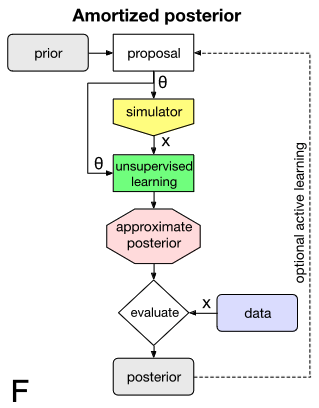
\includegraphics[height=0.6\textheight]{"images/SNPE.png"}
                \caption{\cite{cranmer_frontier_2020}}
            \end{figure}
        \end{column}
    \end{columns}
    

    % Once it's trained you've got your posterior ready to go.

\end{frame}

%%%%%%%%%%%%%%%%%%%%%%%%%%%%%%%
\begin{frame}{Neural Likelihood Estimation (NLE)}
    \begin{columns}
        \begin{column}{0.5\textwidth}
            Model the likelihood rather than the posterior.
    
            \begin{enumerate}[<+->]
                \item Train a neural network $q_\phi$ to approximate $p(x|\theta)$ by maximising $\sum_{i=1}^n \log q_\phi(x_i | \theta_i)$.
        
                
                \item Once $q_\phi$ is trained, proceed by using your likelihood in MCMC to obtain posterior samples.
                
            \end{enumerate}
            \parencite{papamakarios_sequential_2019}
        \end{column}

        \begin{column}{0.5\textwidth}
            \begin{figure}
                \centering
                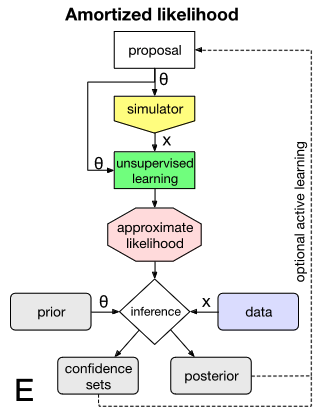
\includegraphics[height=0.6\textheight]{"images/SNLE.png"}
                \caption{\cite{cranmer_frontier_2020}}
            \end{figure}
        \end{column}
    \end{columns}

\end{frame}

%%%%%%%%%%%%%%%%%%%%%%%%%%%%%%%
\section{Sequential Algorithms}
\begin{frame}{Problems with NPE \& NLE}
    \begin{itemize}[<+->]
        \item NPE \& NLE require a lot of data to accurately describe the posterior everywhere.
        \item But we might only want to learn the posterior in parameter- and data-space relevant to our real-world observations $x_o$.
        \item \alert{Solution}: sequentially choose where in $\Theta$ our next training pair $(\theta_i, x_i)$ should come from so as to be maximally informative.
    \end{itemize}
\end{frame}

%%%%%%%%%%%%%%%%%%%%%%%%%%%%%%%
\begin{frame}{SNPE (Type A)}
\begin{itemize}[<+->]
    \item Instead of drawing $\theta \sim p(\theta)$ for each training example, draw from some other proposal distribution $\tilde{p}(\theta)$.
    \begin{itemize}
        \item Such as the current posterior approximation $q_\phi(\theta | x_o)$! 
        \item (Update this proposal every $N \in \mathbb{N}$ samples.)
    \end{itemize}

    \item \alert{Problem}: This would end up biasing us away from the true posterior $p(\theta | x_o) \propto p(x_o|\theta)p(\theta)$ and toward $p(\theta | x_o) \tilde{p}(\theta)$ (ignoring normalisation).

    \item \alert{Solution}: Model the posterior as $p(\theta | x = x_o) \approx \frac{p(\theta)}{\tilde{p}(\theta)}q_\phi(\theta | x_o)$. \parencite{papamakarios_fast_2018}
\end{itemize}

\end{frame}

%%%%%%%%%%%%%%%%%%%%%%%%%%%%%%%
\begin{frame}{SNPE (Type A)}
    \begin{columns}
        \begin{column}{0.67\textwidth}
            \begin{figure}
                \centering
                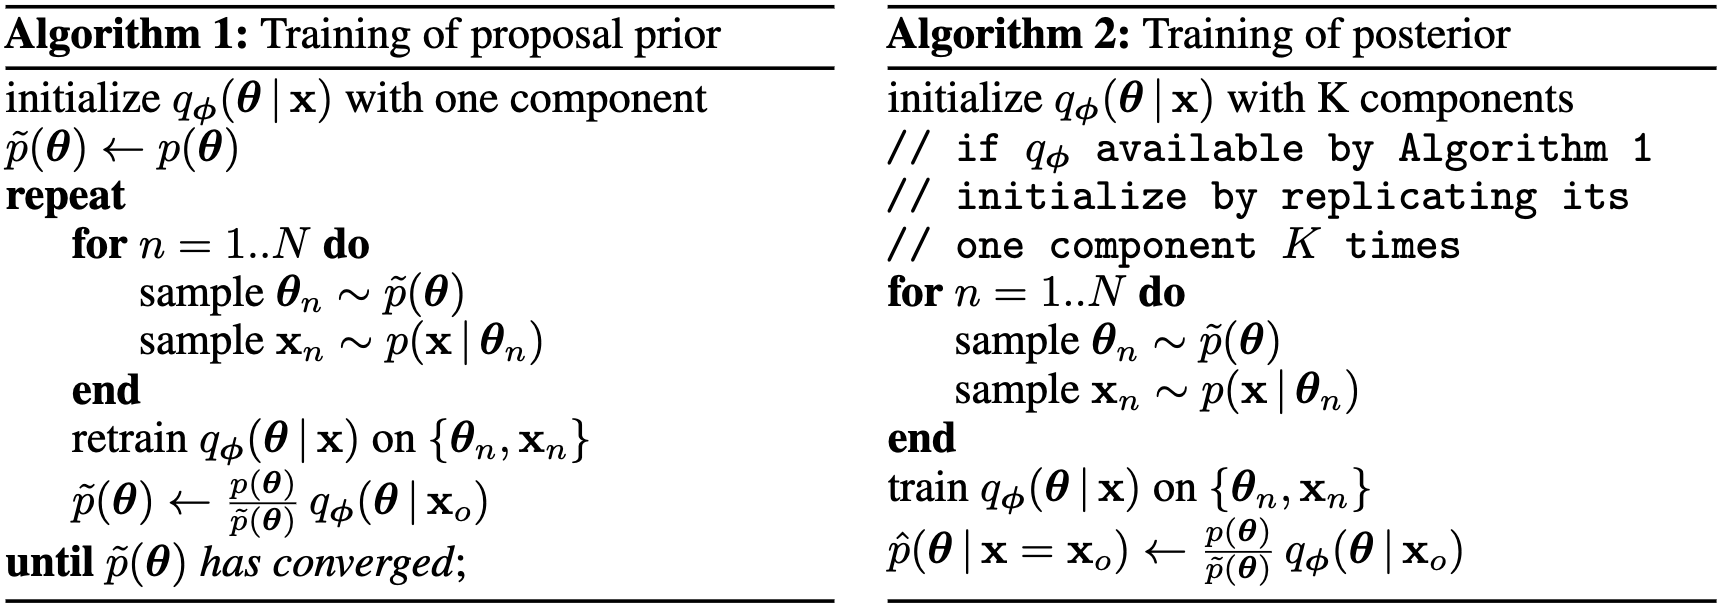
\includegraphics[width=\textwidth]{"images/SNPE_algo2.png"}
                \caption{\cite{hermans_likelihood-free_2020}}
            \end{figure}
        \end{column}

        \begin{column}{0.33\textwidth}
            \begin{figure}
                \centering
                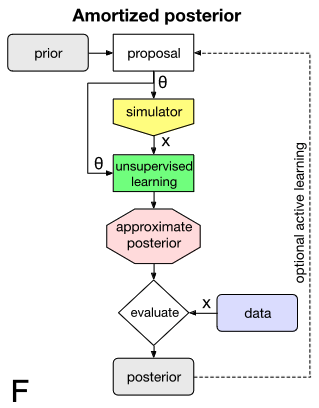
\includegraphics[height=0.6\textheight]{"images/SNPE.png"}
                \caption{\cite{cranmer_frontier_2020}}
            \end{figure}
        \end{column}
    \end{columns}
\end{frame}

% %%%%%%%%%%%%%%%%%%%%%%%%%%%%%%%
% \begin{frame}{SNPE (Type A)}
% [RESULTS SCREENSHOT]
% \end{frame}

%%%%%%%%%%%%%%%%%%%%%%%%%%%%%%%
\begin{frame}{SNPE (Type B)}
\begin{itemize}[<+->]
    \item SNPE-A works, but the division $\frac{p(\theta)}{\tilde{p}(\theta)}$ can be numerically unstable.
    \item \alert{Solution}: use importance weights $w_i = \frac{p(\theta_i)}{\tilde{p}(\theta_i)}$ in your NN objective \parencite{lueckmann_flexible_2017}:
    $$\sum_{i=1}^n w_i \log q_\phi(\theta_i | x_i)$$

    \item (Though often $w_i$ have high variance $\to$ NN gradients have high variance $\to$ training instability.)
\end{itemize}
% This works but can lead to numerical instability if any components of $\tilde{p}$ have smaller variance than $\tilde{p}$---if both are Gaussians then $\frac{p(\theta)}{\tilde{p}(\theta)}$ becomes a Gaussian with negative variance.

\end{frame}

% %%%%%%%%%%%%%%%%%%%%%%%%%%%%%%%
% \begin{frame}{SNPE (Type B)}
%     \begin{columns}
%         \begin{column}{0.5\textwidth}
%             \begin{figure}
%                 \centering
%                 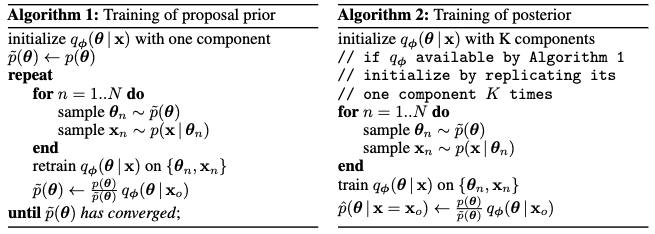
\includegraphics[height=0.7\textheight]{"images/SNPE_algo.png"}
%                 \caption{\cite{hermans_likelihood-free_2020}}
%             \end{figure}
%         \end{column}

%         \begin{column}{0.5\textwidth}
%             \begin{figure}
%                 \centering
%                 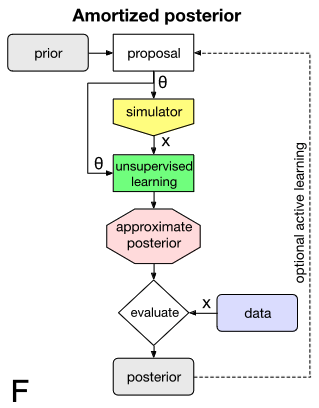
\includegraphics[height=0.7\textheight]{"images/SNPE.png"}
%                 \caption{\cite{cranmer_frontier_2020}}
%             \end{figure}
%         \end{column}
%     \end{columns}
% \end{frame}

% %%%%%%%%%%%%%%%%%%%%%%%%%%%%%%%
% \begin{frame}{SNPE (Type B)}
% [RESULTS SCREENSHOT]
% \end{frame}

%%%%%%%%%%%%%%%%%%%%%%%%%%%%%%%
\begin{frame}{SNLE}
\begin{columns}
    \begin{column}{0.5\textwidth}
        \begin{itemize}[<+->]
            \item Essentially the same thing but have $q_\phi$ model the likelihood.
            % \parencite{papamakarios_sequential_2019}.
            \begin{itemize}
                \item Avoids the posterior-bias problems.
            \end{itemize}
            % \item Two alterations we have to make:
            % \begin{enumerate}
                \item Note: $q_\phi$ is no longer a posterior, so we have to sample our $\theta_i \sim \tilde{p}(\theta | x_o)$ using MCMC (using $q_\phi (x_o | \theta)$ as our likelihood).
            %     \item We return our posterior as $\tilde{p}(\theta | x_o) \propto q_\phi (x_o | \theta)p(\theta)$
            % \end{enumerate}
        \end{itemize}
    \end{column}
        
    \begin{column}{0.5\textwidth}
        \begin{figure}
            \centering
            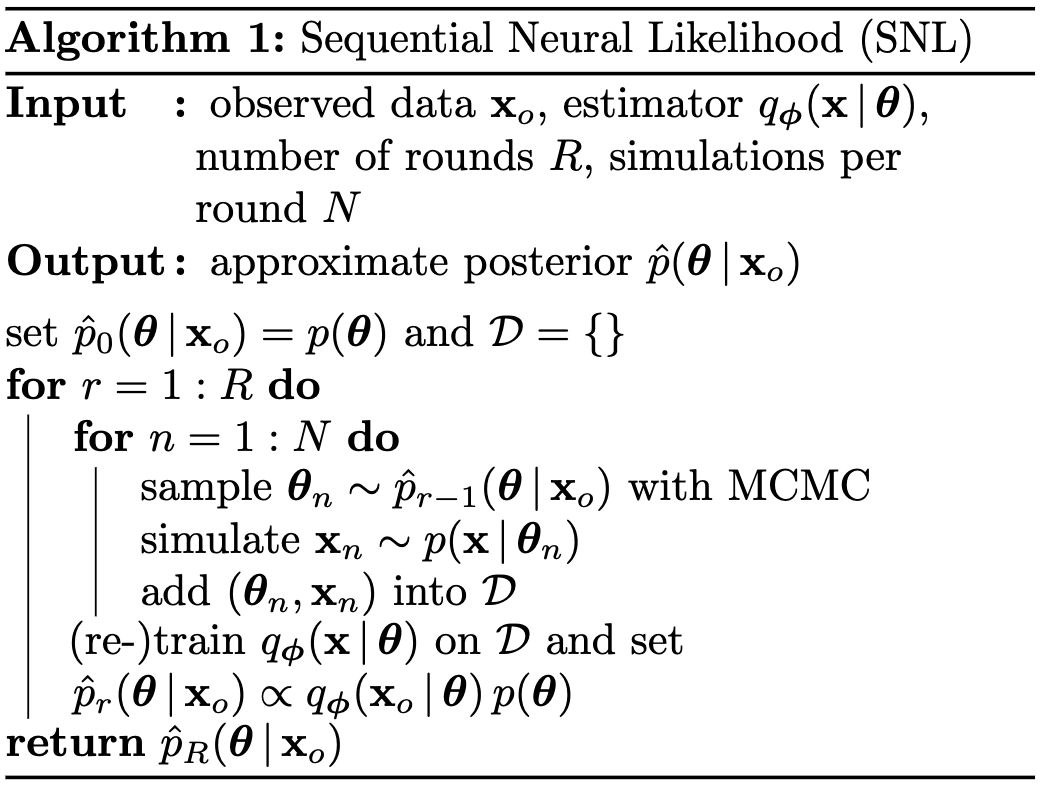
\includegraphics[height=0.6\textheight]{"images/SNLE_algo2.png"}
            \caption{\cite{papamakarios_sequential_2019}}
        \end{figure}
    \end{column}
\end{columns}
    

\end{frame}

%%%%%%%%%%%%%%%%%%%%%%%%%%%%%%%
\begin{frame}{SNLE}
    \begin{figure}
        \centering
        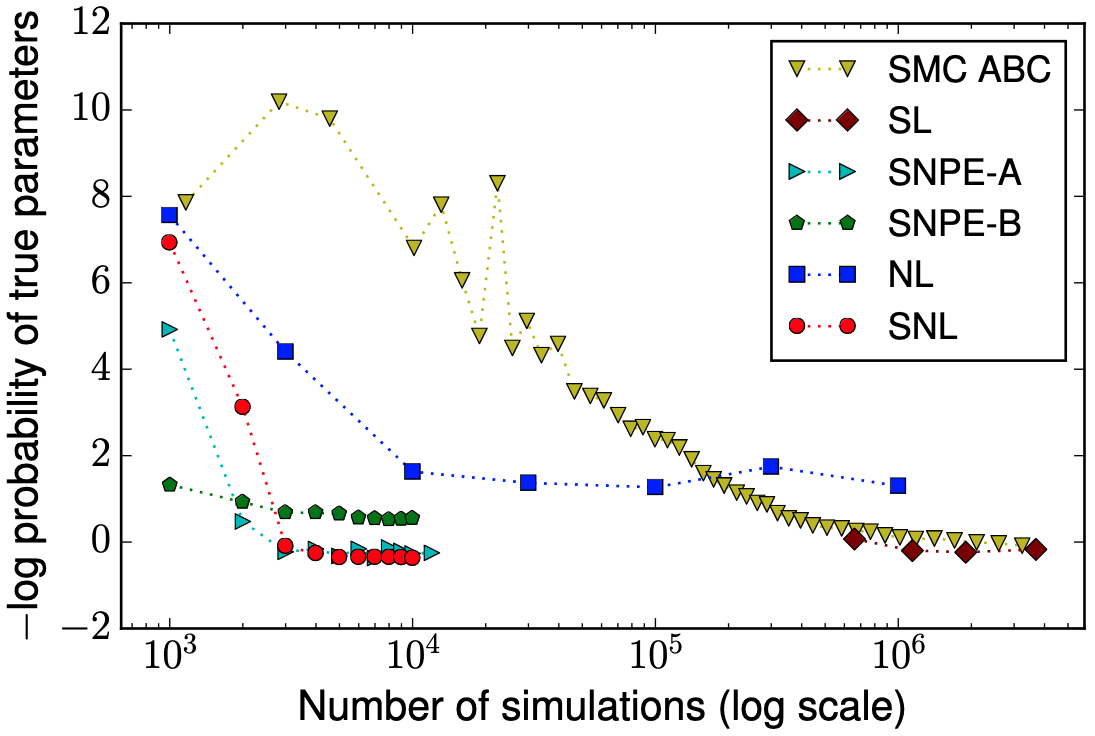
\includegraphics[height=0.7\textheight]{"images/SNLE_results2.png"}
        \caption{\cite{papamakarios_sequential_2019}}
    \end{figure}
\end{frame}


%%%%%%%%%%%%%%%%%%%%%%%%%%%%%%%
\begin{frame}{SNRE}
We can use this idea of sampling from the current approximation to the posterior to help us generate training data for NRE too! \parencite{durkan_contrastive_2020}
\end{frame}

% Probably no algorithm screenshot for SNRE --- it's a big grim

%%%%%%%%%%%%%%%%%%%%%%%%%%%%%%%
\section{Comparison}
% \begin{frame}{Comparison of Algorithms}
%     \begin{figure}
%         \centering
%         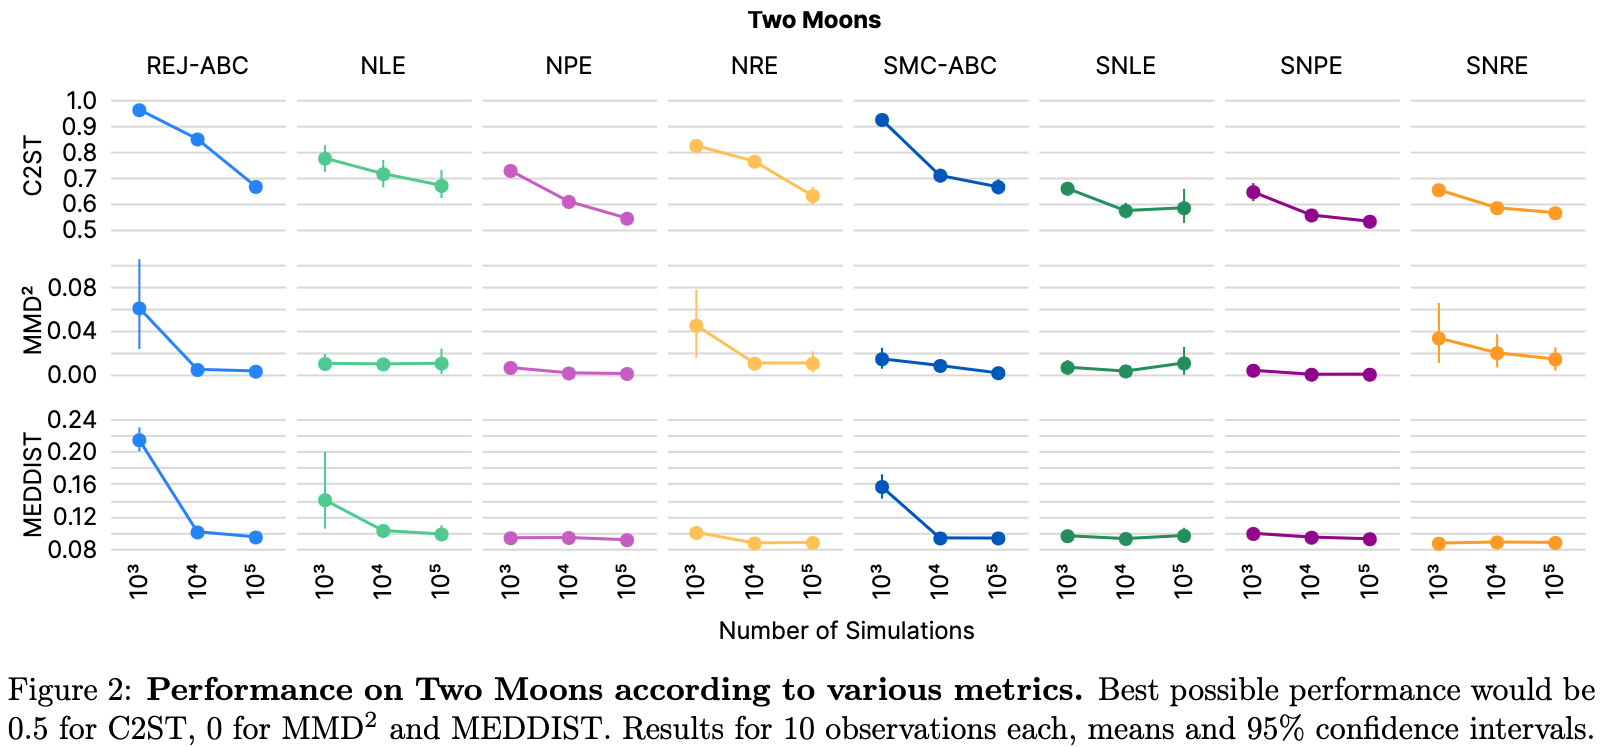
\includegraphics[width=0.8\textwidth]{"images/benchmarking_results_2moons2.png"}
%         \caption{\cite{lueckmann_benchmarking_2021}}
%     \end{figure}
% \end{frame}

% %%%%%%%%%%%%%%%%%%%%%%%%%%%%%%%
% \section{Comparison}
\begin{frame}{Comparison of Algorithms}
    \begin{columns}
        \begin{column}{0.9\textwidth}
            \begin{figure}
                \centering
                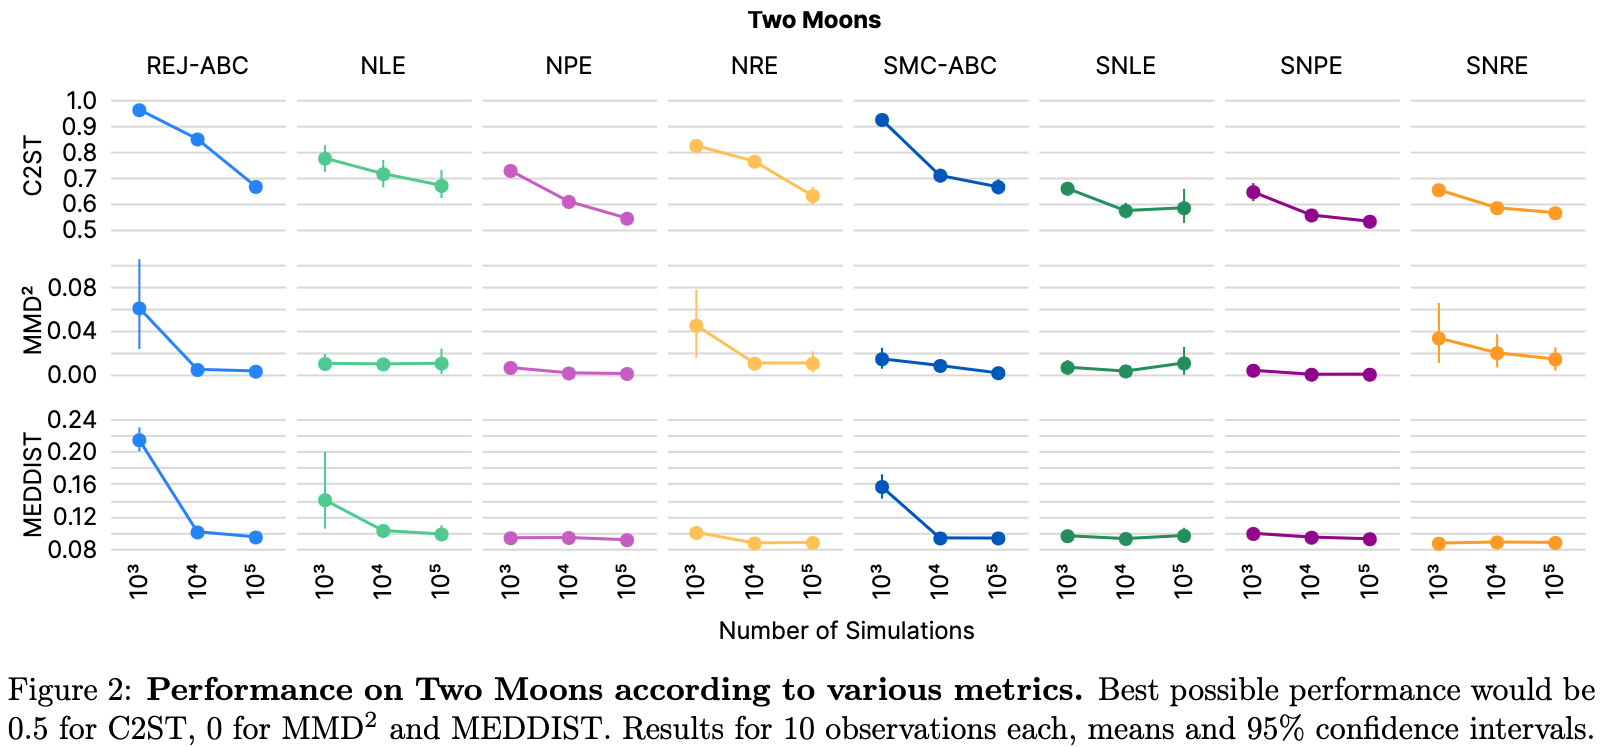
\includegraphics[width=0.87\textwidth]{"images/benchmarking_results_2moons2.png"}
                \caption{\cite{lueckmann_benchmarking_2021}}
            \end{figure}
        \end{column}

        \begin{column}{0.1\textwidth}
            \begin{figure}
                \centering
                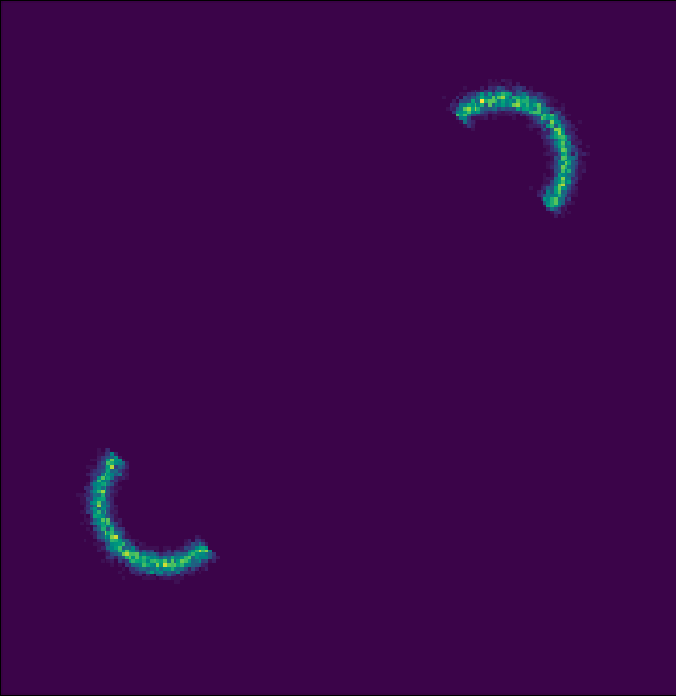
\includegraphics[width=\textwidth]{"images/2moons.png"}
                \caption{\cite{sharrock_sequential_2022}}
            \end{figure}
        \end{column}
    \end{columns}
   
\end{frame}

% %%%%%%%%%%%%%%%%%%%%%%%%%%%%%%%
% \begin{frame}{Comparison of Algorithms}
% \begin{figure}
%         \centering
%         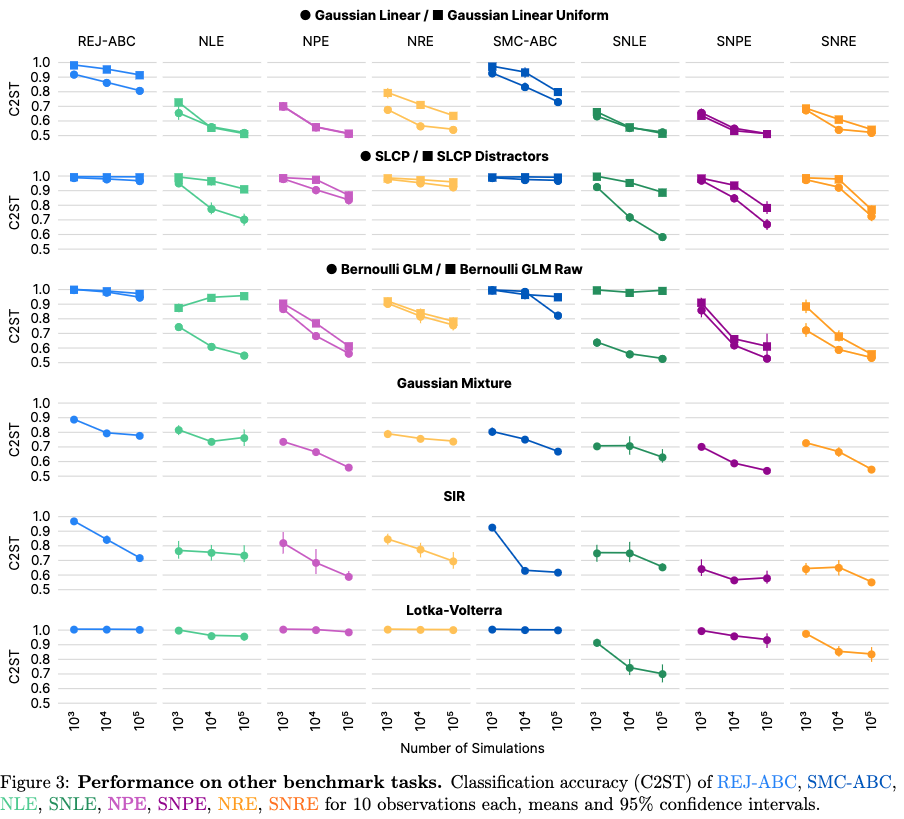
\includegraphics[height=0.8\textheight]{"images/benchmarking_results_more.png"}
%         \caption{\cite{lueckmann_benchmarking_2021}}
%     \end{figure}
% \end{frame}

%%%%%%%%%%%%%%%%%%%%%%%%%%%%%%%
\begin{frame}{Comparison of Algorithms}
\begin{figure}
        \centering
        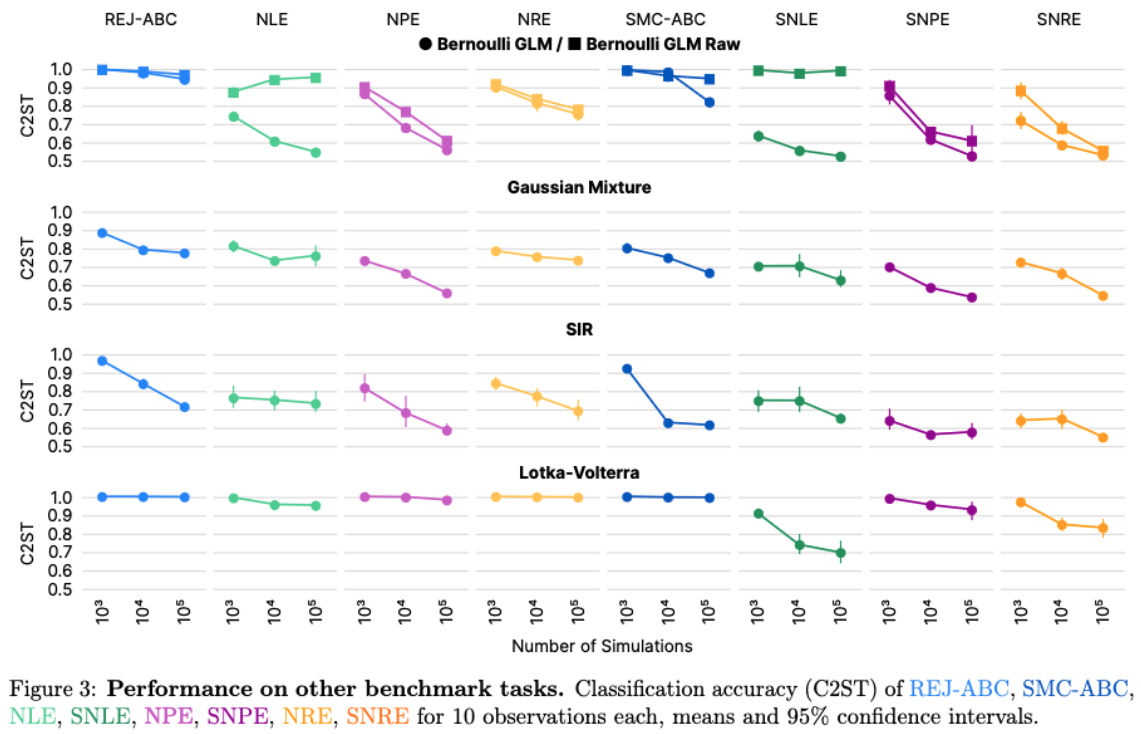
\includegraphics[height=0.8\textheight]{"images/benchmarking_results_more_compact.png"}
        \caption{\cite{lueckmann_benchmarking_2021}}
    \end{figure}
\end{frame}

%%%%%%%%%%%%%%%%%%%%%%%%%%%%%%%
\begin{frame}{Comparison of Algorithms}
What each algorithm gives you:
\pause
\begin{itemize}
    \item ABC: 
    \begin{itemize}
        \item Samples from posterior $\theta \sim q(\theta|x_o)$.
    \end{itemize}
    
    \pause
    
    \item (S)NLE + (S)NRE:
    \begin{itemize}
        \item Samples from posterior $\theta \sim q(\theta|x_o)$ via MCMC.
        \item Unnormalised evaluations $q(\theta|x_o)$.
    \end{itemize}
    
    \pause
    
    \item (S)NPE:
    \begin{itemize}
        \item Samples from posterior $\theta \sim q(\theta|x_o)$ directly.
        \item Normalised evaluations $q(\theta|x_o)$.
    \end{itemize}
    
\end{itemize}
\end{frame}

%%%%%%%%%%%%%%%%%%%%%%%%%%%%%%%
\begin{frame}{Comparison of Algorithms}
\begin{itemize}[<+->]
    \item Different problems lend themselves to different algorithms as solutions...

    \item Sequential algorithms might not always be best:
    \begin{itemize}
        \item Not needed if simulation is cheap.

        \item Performing SBI separately for many data points:
        \begin{itemize}
            \item Better to have an amortized likelihood/posterior that is accurate everywhere in the data-space $x_o \in \mathcal{X}$.
            \item E.g. for iid data $x_{o_1}, x_{o_2} \ldots \sim p(x | \theta)$
            $$p(\theta | x_{o_1}, x_{o_2} \ldots) \propto p(\theta) \prod_i \left[\underbrace{p(x_{o_i} | \theta)}_{\text{amortized likelihood}}\right].$$
        \end{itemize}
        % \begin{itemize}
        %     \item  iid (compute $p(\theta|x_{o_1}), p(\theta|x_{o_2}), \ldots$)
        %     \item Amortized methods (NPE) probably preferable.
        %     \item (Amortised likelihoods (NRE/NLE) require MCMC sampling.)
        % \end{itemize}
        
        % \item Performing SBI on lots of iid data (compute $p(\theta|x_{o_1}, x_{o_2}, \ldots)$)
        % \begin{itemize}
        %     \item Better to have an amortized likelihood/posterior that is accurate everywhere in the data-space $x_o \in \mathcal{X}$.
        % \end{itemize}
    \end{itemize}
\end{itemize}
\end{frame}


%%%%%%%%%%%%%%%%%%%%%%%%%%%%%%%
\section{Conclusion}
\begin{frame}{Conclusion}
\begin{itemize}[<+->]
    \item SNPE/SNLE/SNRE are all pretty popular, but there are other methods out there too, e.g.:
    \begin{itemize}
        \item GATSBI \parencite{ramesh_gatsbi_2022} --- GAN-inspired approach.
        \item `Grey-box' approaches \parencite{brehmer_mining_2020} --- try to squeeze as much information out of the simulator as possible.
    \end{itemize}
    \item SBI is pretty promising for a whole range of scientific subjects
    \begin{itemize}
        \item Particle physics \parencite{brehmer_simulation-based_2020}.
        \item Astrophysics --- gravitational waves \parencite{delaunoy_lightning-fast_2020}, dark matter \parencite{hermans_towards_2021}.
        \item Climate science --- hydrology of river basins in Colorado \cite{hull_using_2022}.
    \end{itemize}
\end{itemize}
\end{frame}

%%%%%%%%%%%%%%%%%%%%%%%%%%%%%%%
\begin{frame}{Useful Papers}
    \begin{figure}
        \centering
        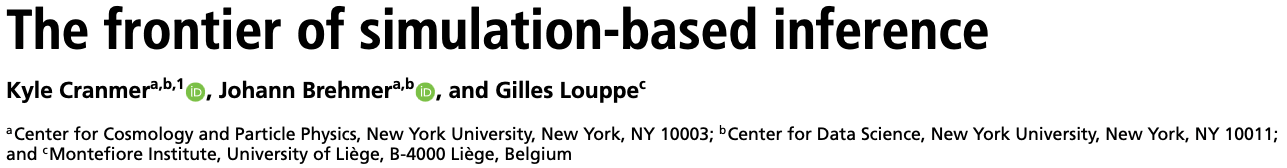
\includegraphics[height=0.25\textheight]{"images/review_header.png"}
        % \caption{\cite{cranmer_frontier_2020}}
    \end{figure}
    
    \vspace{1em}
    
    \begin{figure}
        \centering
        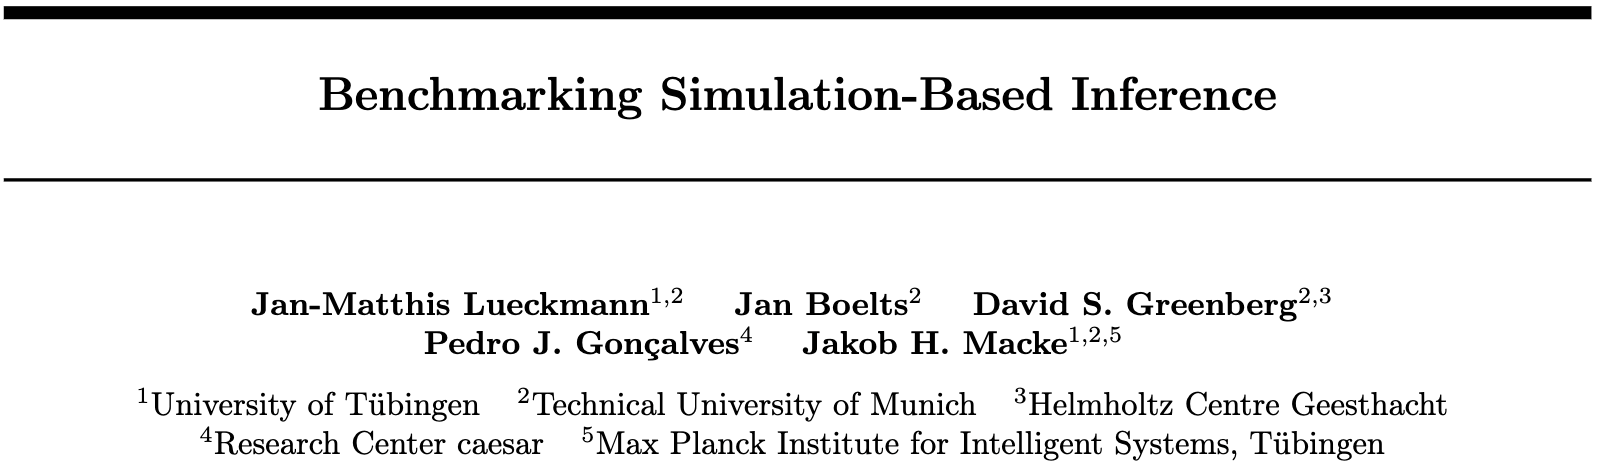
\includegraphics[height=0.4\textheight]{"images/benchmarking_header2.png"}
        % \caption{\cite{lueckmann_benchmarking_2021}}
    \end{figure}
\end{frame}

%%%%%%%%%%%%%%%%%%%%%%%%%%%%%%%
\begin{frame}[allowframebreaks]{References}
    \printbibliography
\end{frame}


\end{document}